\documentclass[11pt]{beamer}

\usetheme{metropolis}

\usepackage{graphicx}
\usepackage{physics}
\usepackage{adjustbox}
\usepackage{caption}
\usepackage{chemformula}
\usepackage{quoting}
\usepackage[style=chem-angew,backend=bibtex]{biblatex}
\bibliography{references}
%
% Choose how your presentation looks.
%
% For more themes, color themes and font themes, see:
% http://deic.uab.es/~iblanes/beamer_gallery/index_by_theme.html
%
\mode<presentation>
{
  \usetheme{default}      % or try Darmstadt, Madrid, Warsaw, ...
  \usecolortheme{default} % or try albatross, beaver, crane, ...
  \usefonttheme{default}  % or try serif, structurebold, ...
  \setbeamertemplate{navigation symbols}{}
  \setbeamertemplate{caption}[numbered]
  \setbeamerfont{footnote}{size=\tiny}
} 

\usepackage[english]{babel}
\usepackage[utf8]{inputenc}
\graphicspath{{../lectureMW/image/}}

\AtBeginSection[]{
\begin{frame}{Outline}
  \tableofcontents[currentsection]
\end{frame}
}

\title{Review Electromagnetic Radiation, Naming, and Chem Equations}
\institute{Chemistry Department, Cypress College}
\date{November 3, 2022}

\begin{document}

\begin{frame}
  \titlepage
\end{frame}

\begin{frame}{Class Announcements}
  \textbf{Lecture}
  \begin{itemize}
  \item Share previous UCI Teaching Evaluation
  \item Hold off on reviewing the Exam and homework 8
  \item Review material from Chs 3 - 6
  \item Quiz and Homework assignment released Fri, Nov 4th at 3pm
  \end{itemize}
\end{frame}

\section{Review: Wavelength and Rydberg Formula}

\begin{frame}{The Wave}
  \centering
  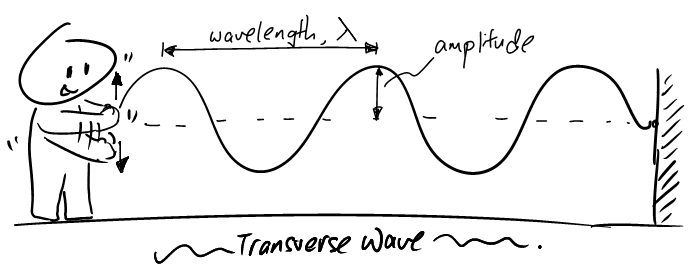
\includegraphics[width=\linewidth]{rope_waves}
\end{frame}

\begin{frame}{Practice: Determining the Wavelength}
  Suppose a 7.5m rope is shaken to yield 2.5 wavelength. Draw the
  wave for 7.5m rope. Determine the wavelength in m.
  \vspace{1.5in}
\end{frame}

\begin{frame}{Rydberg Formula}
  \begin{equation}
    \frac{1}{\lambda} = R\Bigg(\frac{1}{n_f^2} - \frac{1}{n_i^2}\Bigg)
  \end{equation}
  where $n_f$ and $n_i$ are the final and initial energy state,
  $\lambda$ is the wavelength, and $R$ is the Rydberg constant
  ($1.097\times 10^7$ m$^{-1}$)
  \centering
  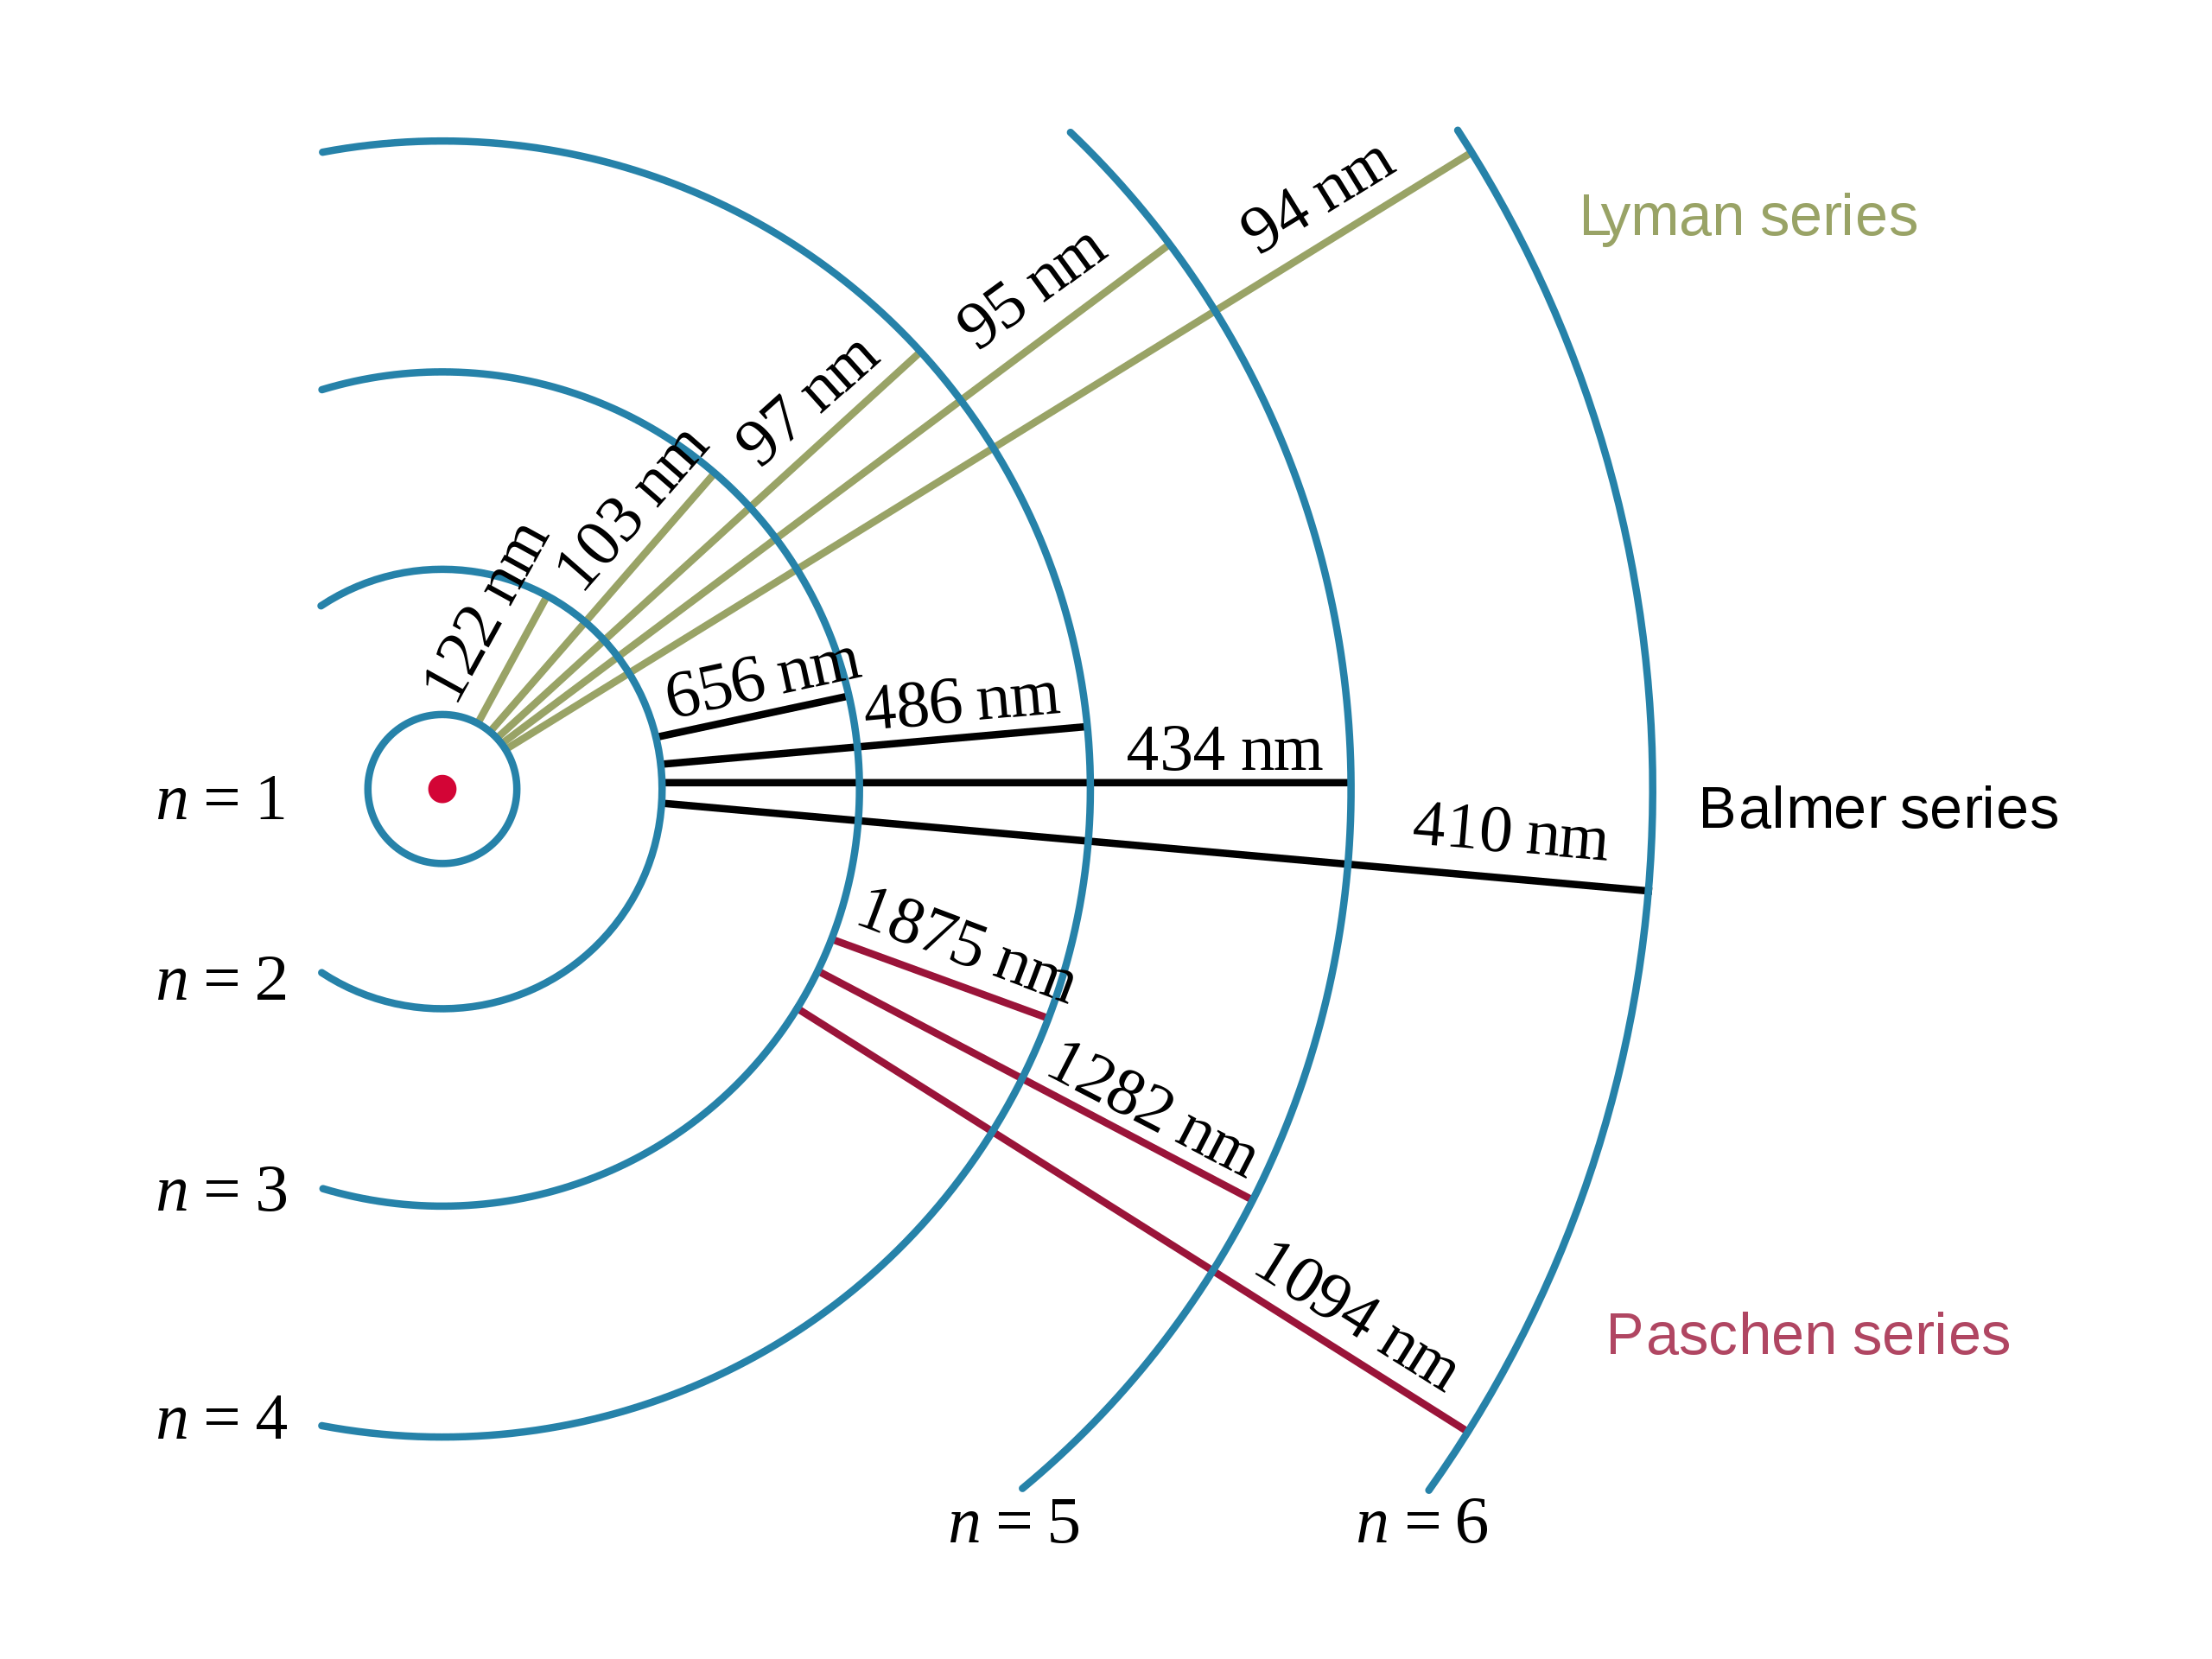
\includegraphics[scale=0.08]{h_spectra}
\end{frame}

\begin{frame}{H Atom Spectra}
  \textbf{Q:} What do notice about the transition energy for n=1 to n=2 and
  n=2 to n=3?
  
  \centering
  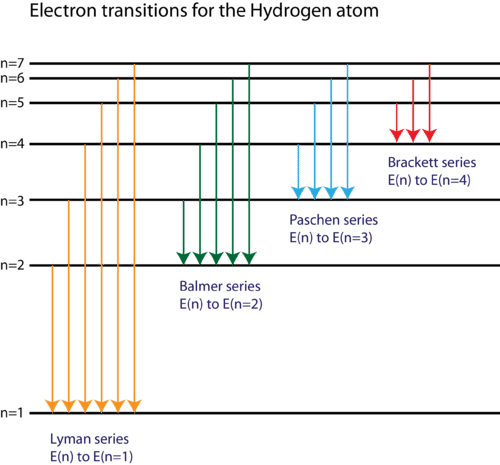
\includegraphics[scale=0.4]{energy_trans_h}
\end{frame}

\section{Review: Identifying Types of Compounds and Naming Compounds}

\begin{frame}{Properties of Ionic Compounds}
  \begin{center}
    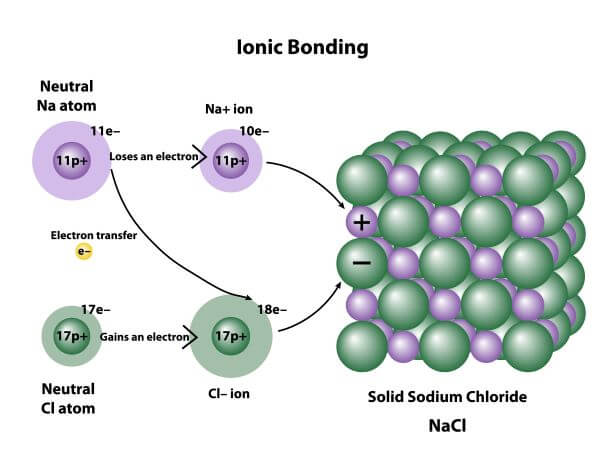
\includegraphics[width=0.6\linewidth]{Ionic-bond-example}
  \end{center}
  \vspace{-0.3in}
  \textbf{Ionic Compounds}
  \begin{itemize}
  \item Highly conductive and strong electrolyte - ability to
    carry electricity (electrons)
  \item High melting and boiling points, high density
  \end{itemize}
\end{frame}

\begin{frame}{Properties of Molecular Compounds}
  \begin{center}
    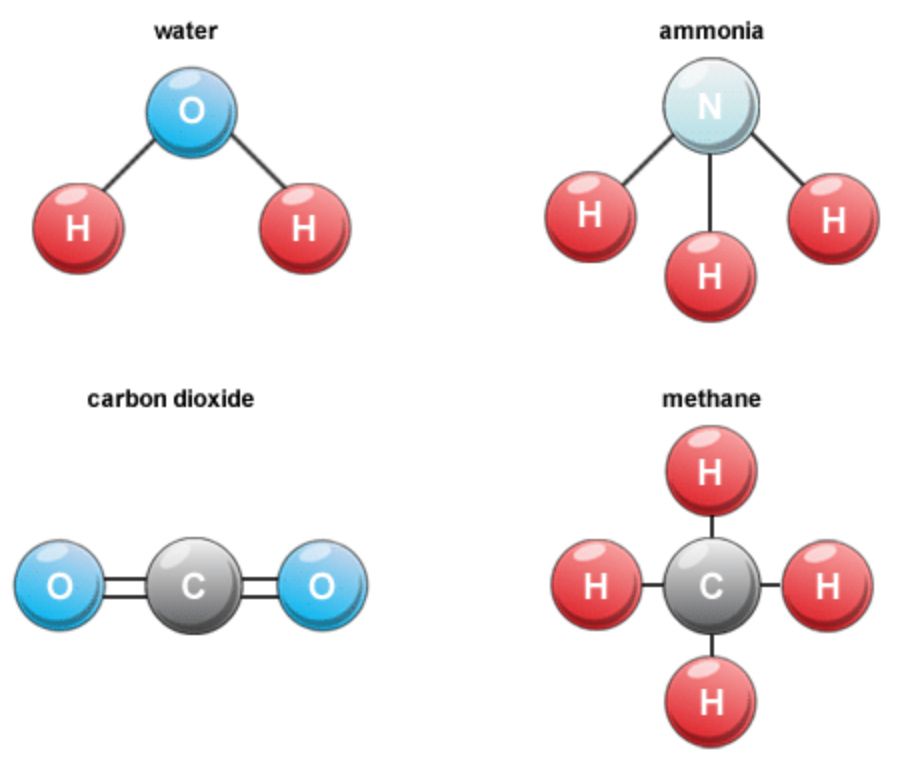
\includegraphics[width=0.6\linewidth]{molec_example}
  \end{center}
  \vspace{-0.3in}
  \textbf{Molecular Compounds}
  \begin{itemize}
  \item Not conductive and weak electrolyte
  \item Low melting and boiling points, low density
  \end{itemize}
\end{frame}

\subsection{Ionic Compounds}

\begin{frame}{Naming Ionic Compounds}
  The metal cation is named first, followed by the nonmetal anion.
  The word ion is dropped from both parts.

  \centering
  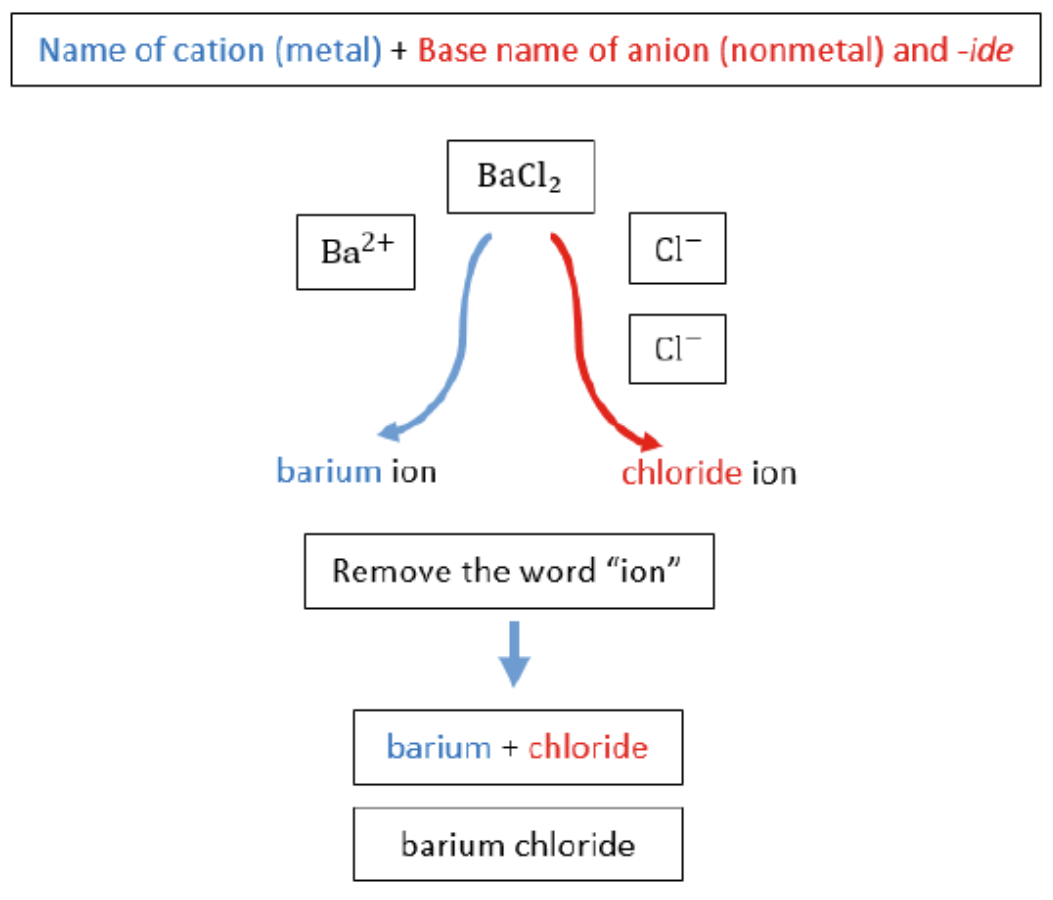
\includegraphics[width=0.7\linewidth]{barium_examp.png}
\end{frame}

\subsection{Molecular Compounds}

\begin{frame}{Naming Molecular Compounds}
  \begin{center}
    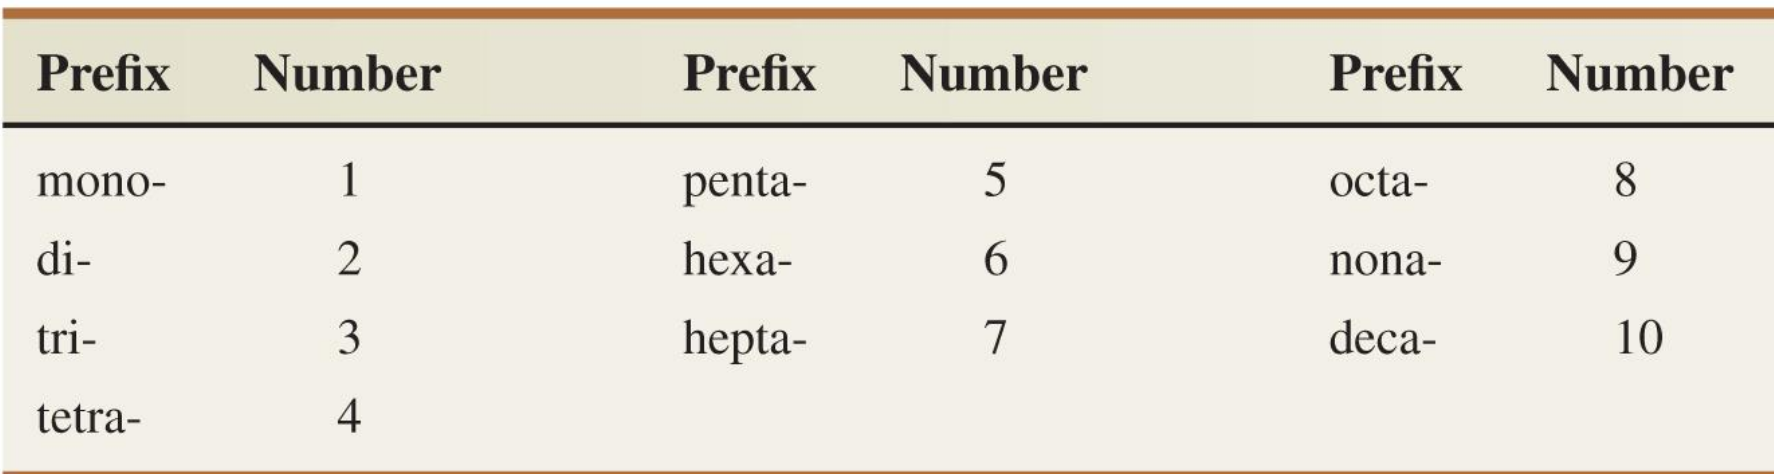
\includegraphics[width=\linewidth]{prefix_name}
  \end{center}
  
  \begin{enumerate}
  \item Use numerical prefix for the element (usually ignore the first
    when using ``mono'')
  \item Add ``-ide'' to the second element
  \end{enumerate}
\end{frame}

\begin{frame}{Practice: Naming Binary Molecular Compounds}
  \begin{itemize}
  \item H$_2$O
  \item N$_2$O$_4$
  \item CO
  \item CH$_4$
  \item PF$_5$
  \item BF$_3$
  \item SiO$_2$
  \item XeF$_4$
  \end{itemize}
\end{frame}

\begin{frame}{Practice: Determining Molecular Formula}
  \begin{itemize}
  \item Sulfur trioxide
  \item Nitrogen trihydride
  \item Dihydrogen monoxide
  \item Carbon tetrafluoride
  \item Selenium dichloride
  \item Dinitrogen pentaoxide
  \item Sulfur hexafluoride
  \item Phosphorus trifluoride
  \end{itemize}
\end{frame}

\subsection{Acids and Bases}

\begin{frame}{Naming Acids and Bases}
  \begin{center}
    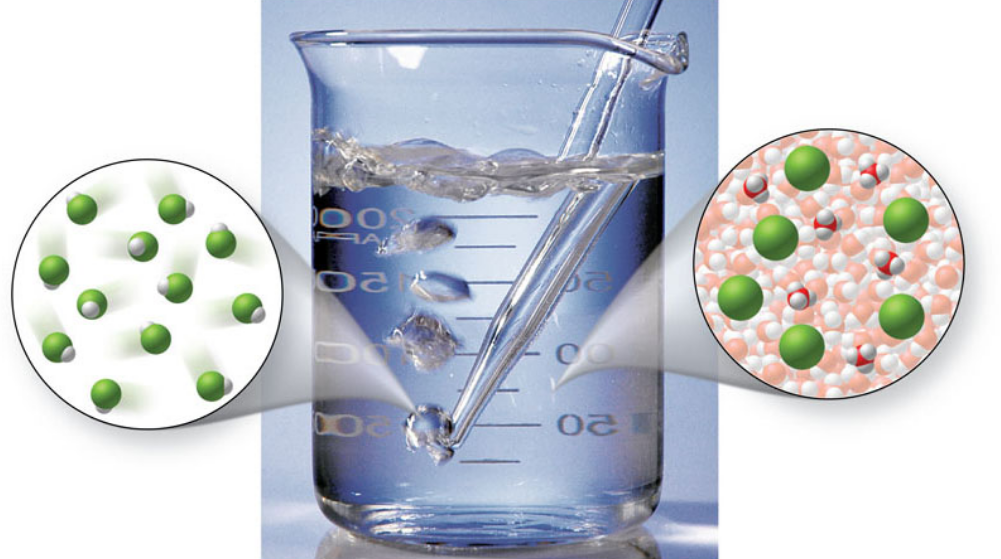
\includegraphics[width=0.5\linewidth]{acid_base}
  \end{center}

  \begin{enumerate}
  \item If anion ends in ``-ide,'' add ``hydro'' before the
    root of the anion name followed by ``-ic acid''
  \item If anion ends in ``-ate,'' use the root of the anion
    name followed by ``-ic acid''
  \item If anion ends in ``-ite,'' use the root of the anion
    name followed by ``-ous acid''
  \end{enumerate}
\end{frame}

\begin{frame}{Practice: Naming the Acid}
  \begin{itemize}
  \item HCl
  \item HNO$_3$
  \item H$_2$CO$_3$
  \item H$_2$SO$_3$
  \item H$_3$PO$_4$
  \item HClO$_2$
  \item HBr
  \item HNO$_2$
  \item H$_2$SO$_3$
  \item H$_2$S
  \end{itemize}
\end{frame}

\begin{frame}{Practice: Determining Molecular Formula}
  \begin{itemize}
  \item Cloric acid
  \item Phosphoric acid
  \item Sulfurous acid
  \item Hydrosulfuric acid
  \item Chromic acid
  \item Nitric acid
  \item Hypochlorous acid
  \item Hydrobromic acid
  \end{itemize}
\end{frame}

\section{Review: Heat and Energy}

\begin{frame}{Endothermic and Exothermic Reactions}
  \centering
  
\includegraphics[width=0.8\linewidth]{exo_endo}

  \textbf{Exo} - external; exothermic reactions give off
  heat

  \textbf{Endo} - internal; endothermic reactions absorb
  heat
\end{frame}

\begin{frame}{Endothermic Reaction Diagram}
  \centering
  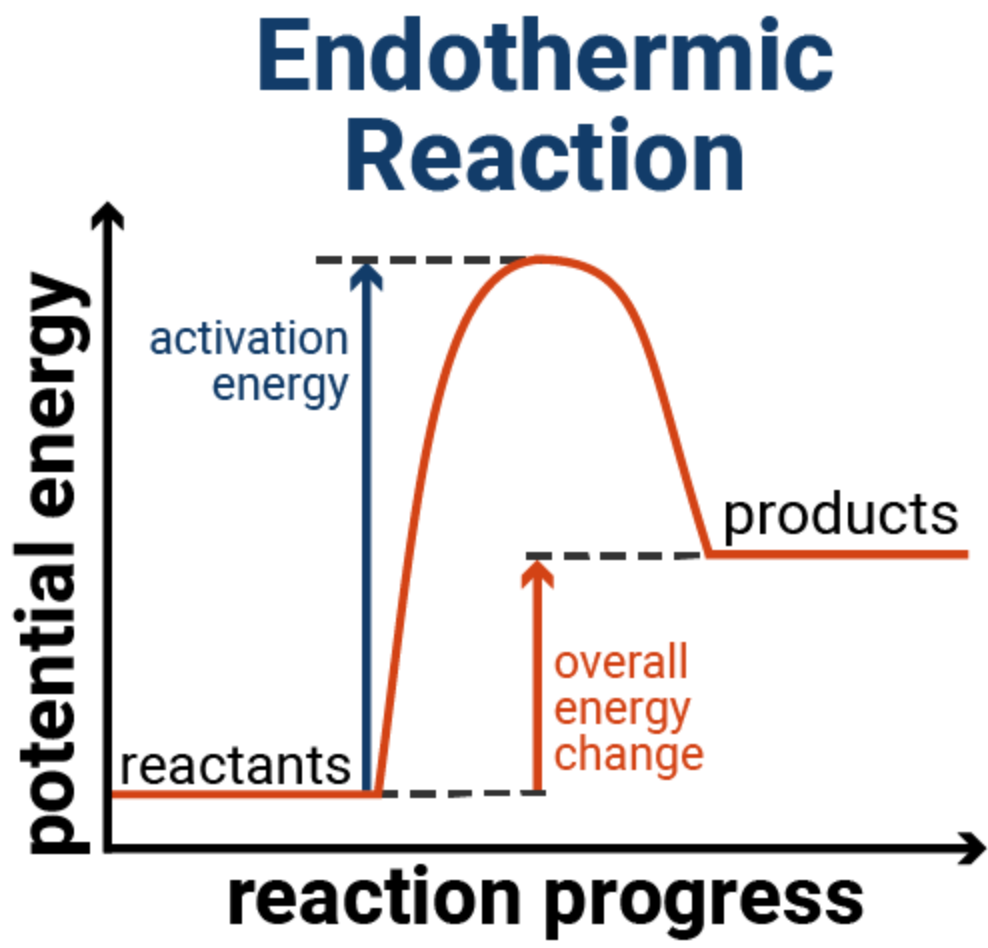
\includegraphics[width=0.5\linewidth]{endo_rxn}

  \begin{itemize}
  \item \textbf{Recall Potential energy} - ability to do
    work; $\Delta E_\text{products} > \Delta E_\text{reactants}$
  \item \textbf{Activation energy} - minimum energy to start the
    reaction; determines the rate at which the reaction undergoes
  \end{itemize}
\end{frame}

\begin{frame}{Examples of Endothermic Reactions}
  \centering
  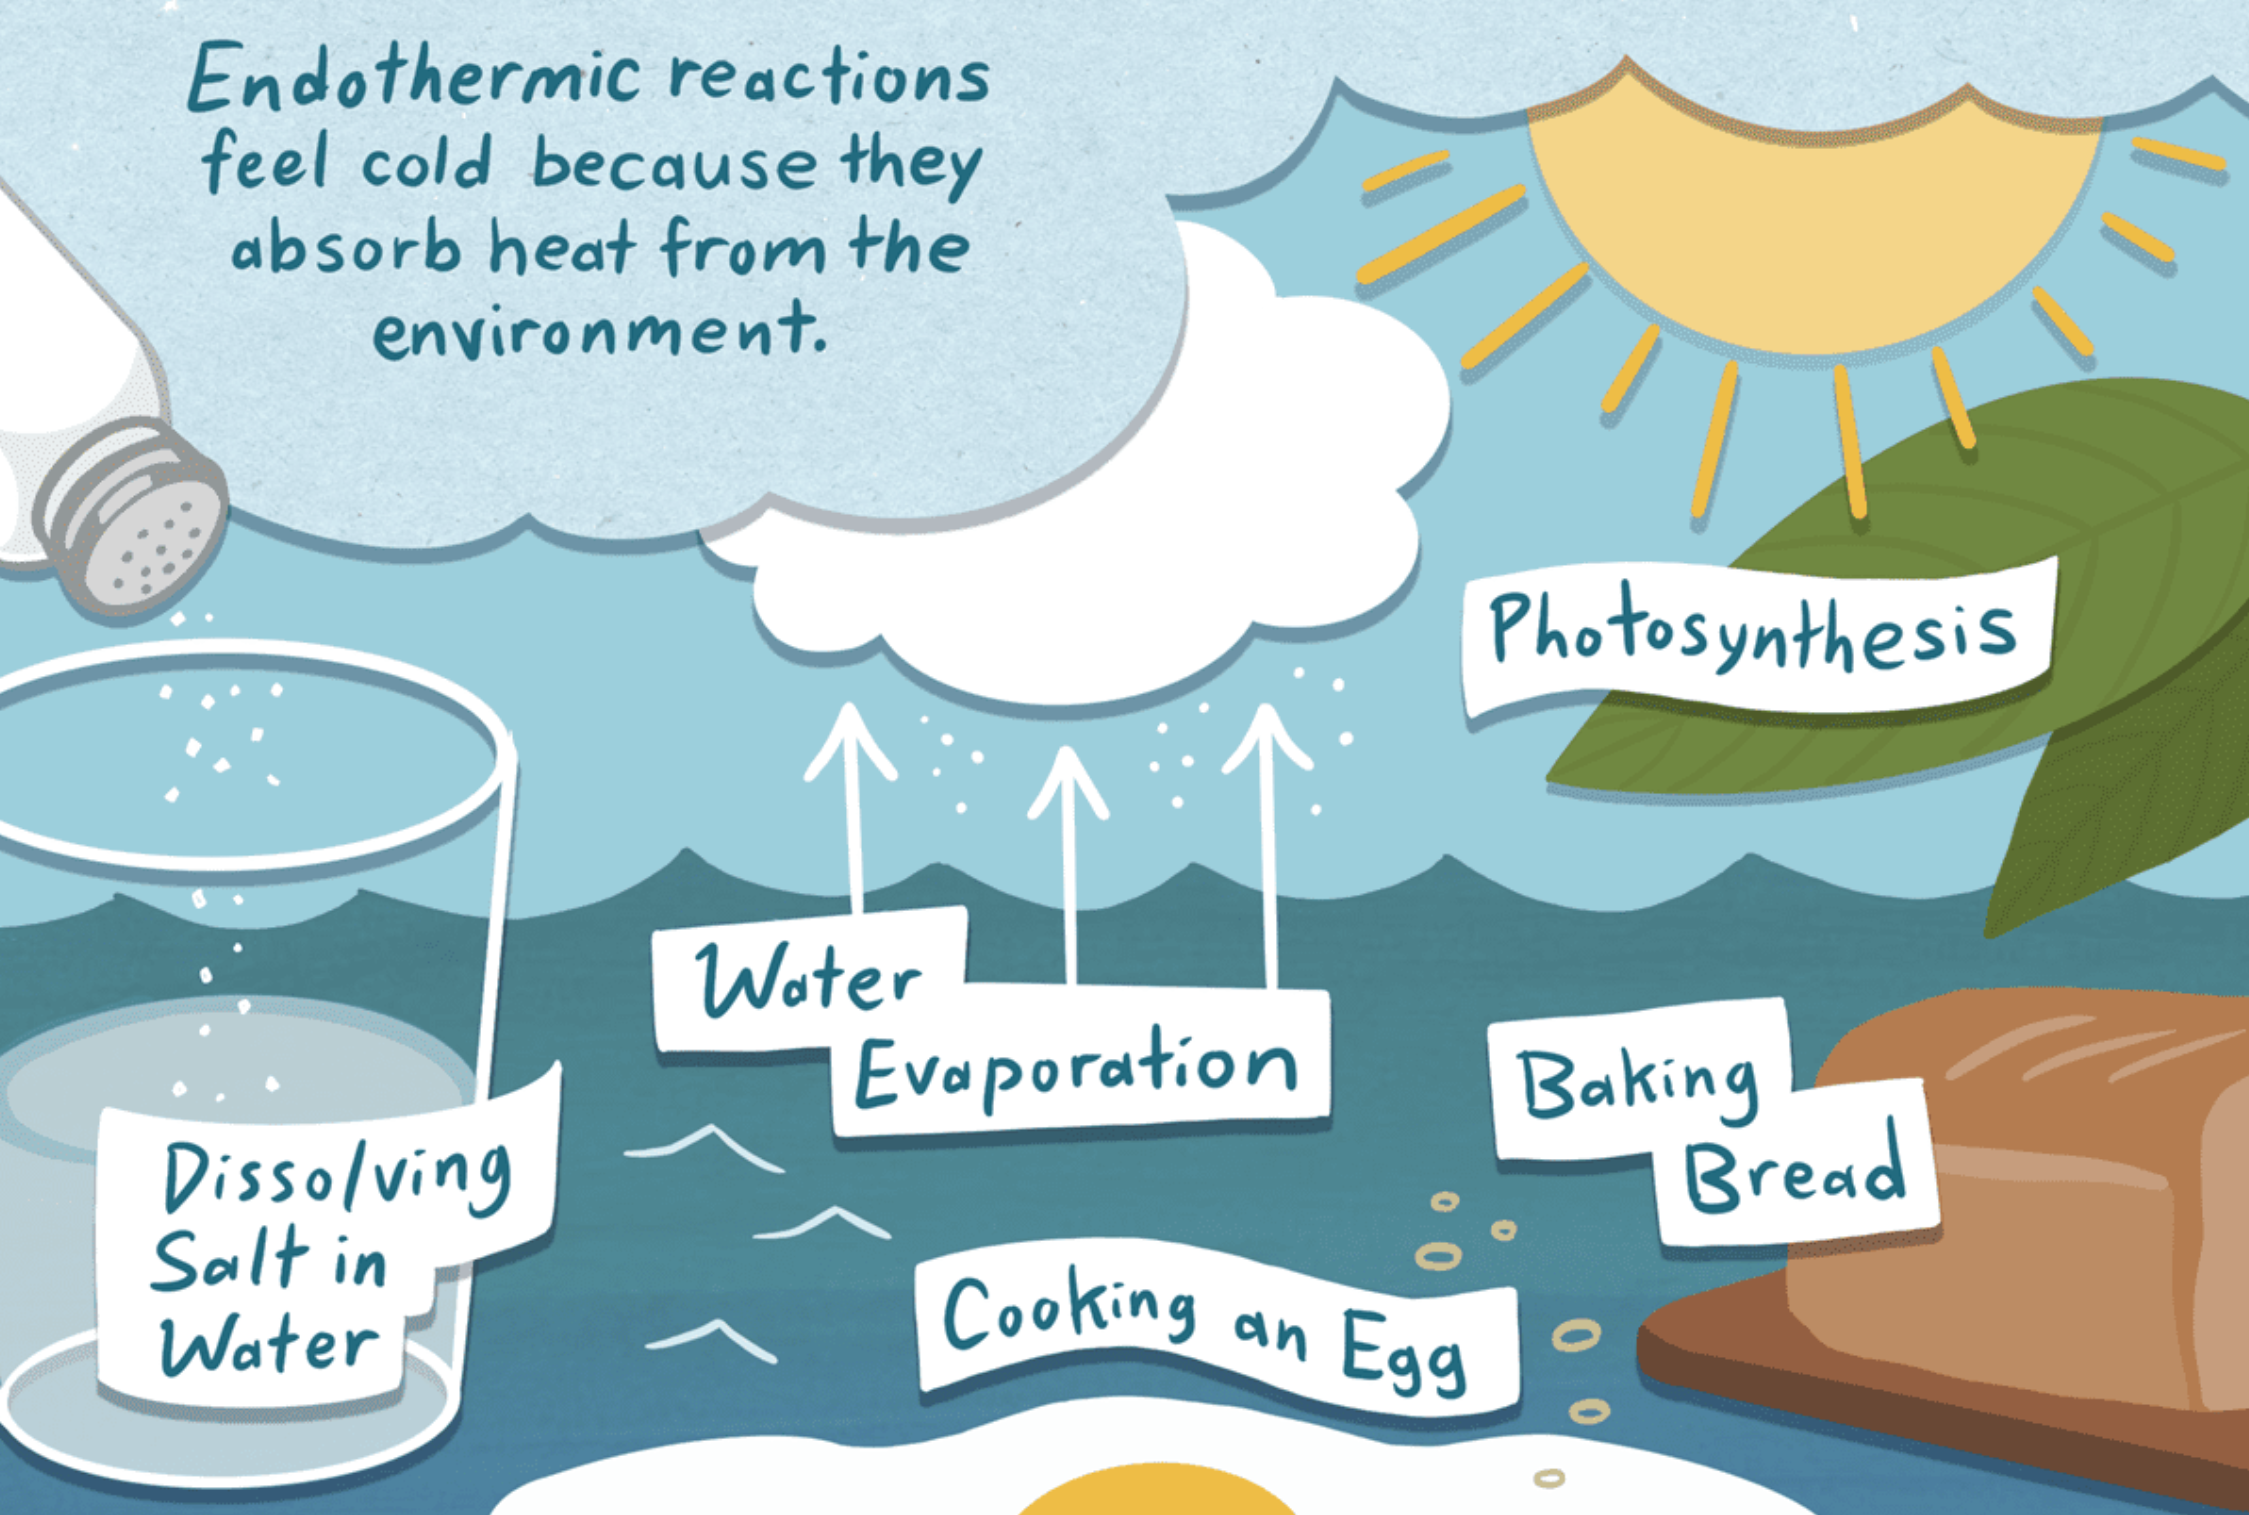
\includegraphics[width=\linewidth]{endo_everyday}
\end{frame}

\begin{frame}{Exothermic Reaction Diagram}
  \centering
  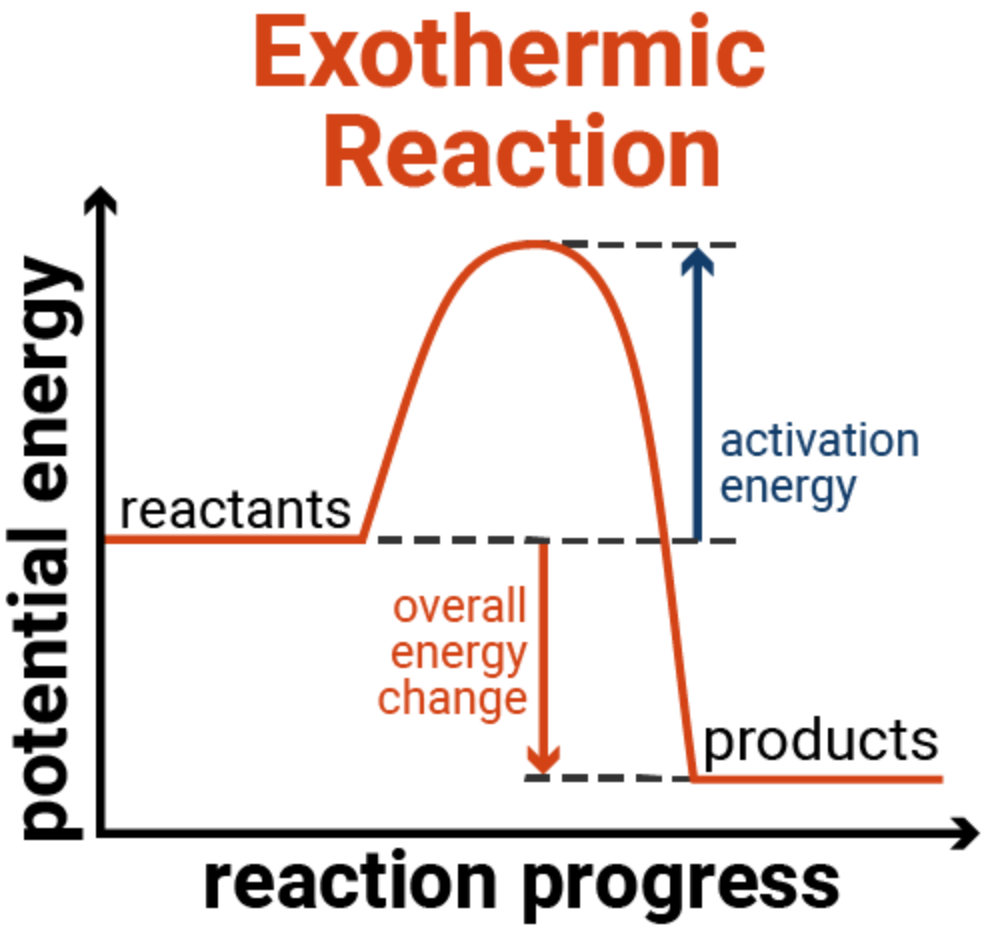
\includegraphics[width=0.5\linewidth]{exo_rxn}
  \begin{itemize}
  \item \textbf{Potential energy} - $\Delta E_\text{products} < \Delta E_\text{reactants}$
  \item Products are more stable than reactants since preference
    for lower energy state
  \end{itemize}
\end{frame}

\begin{frame}{Examples of Exothermic Reactions}
  \centering
  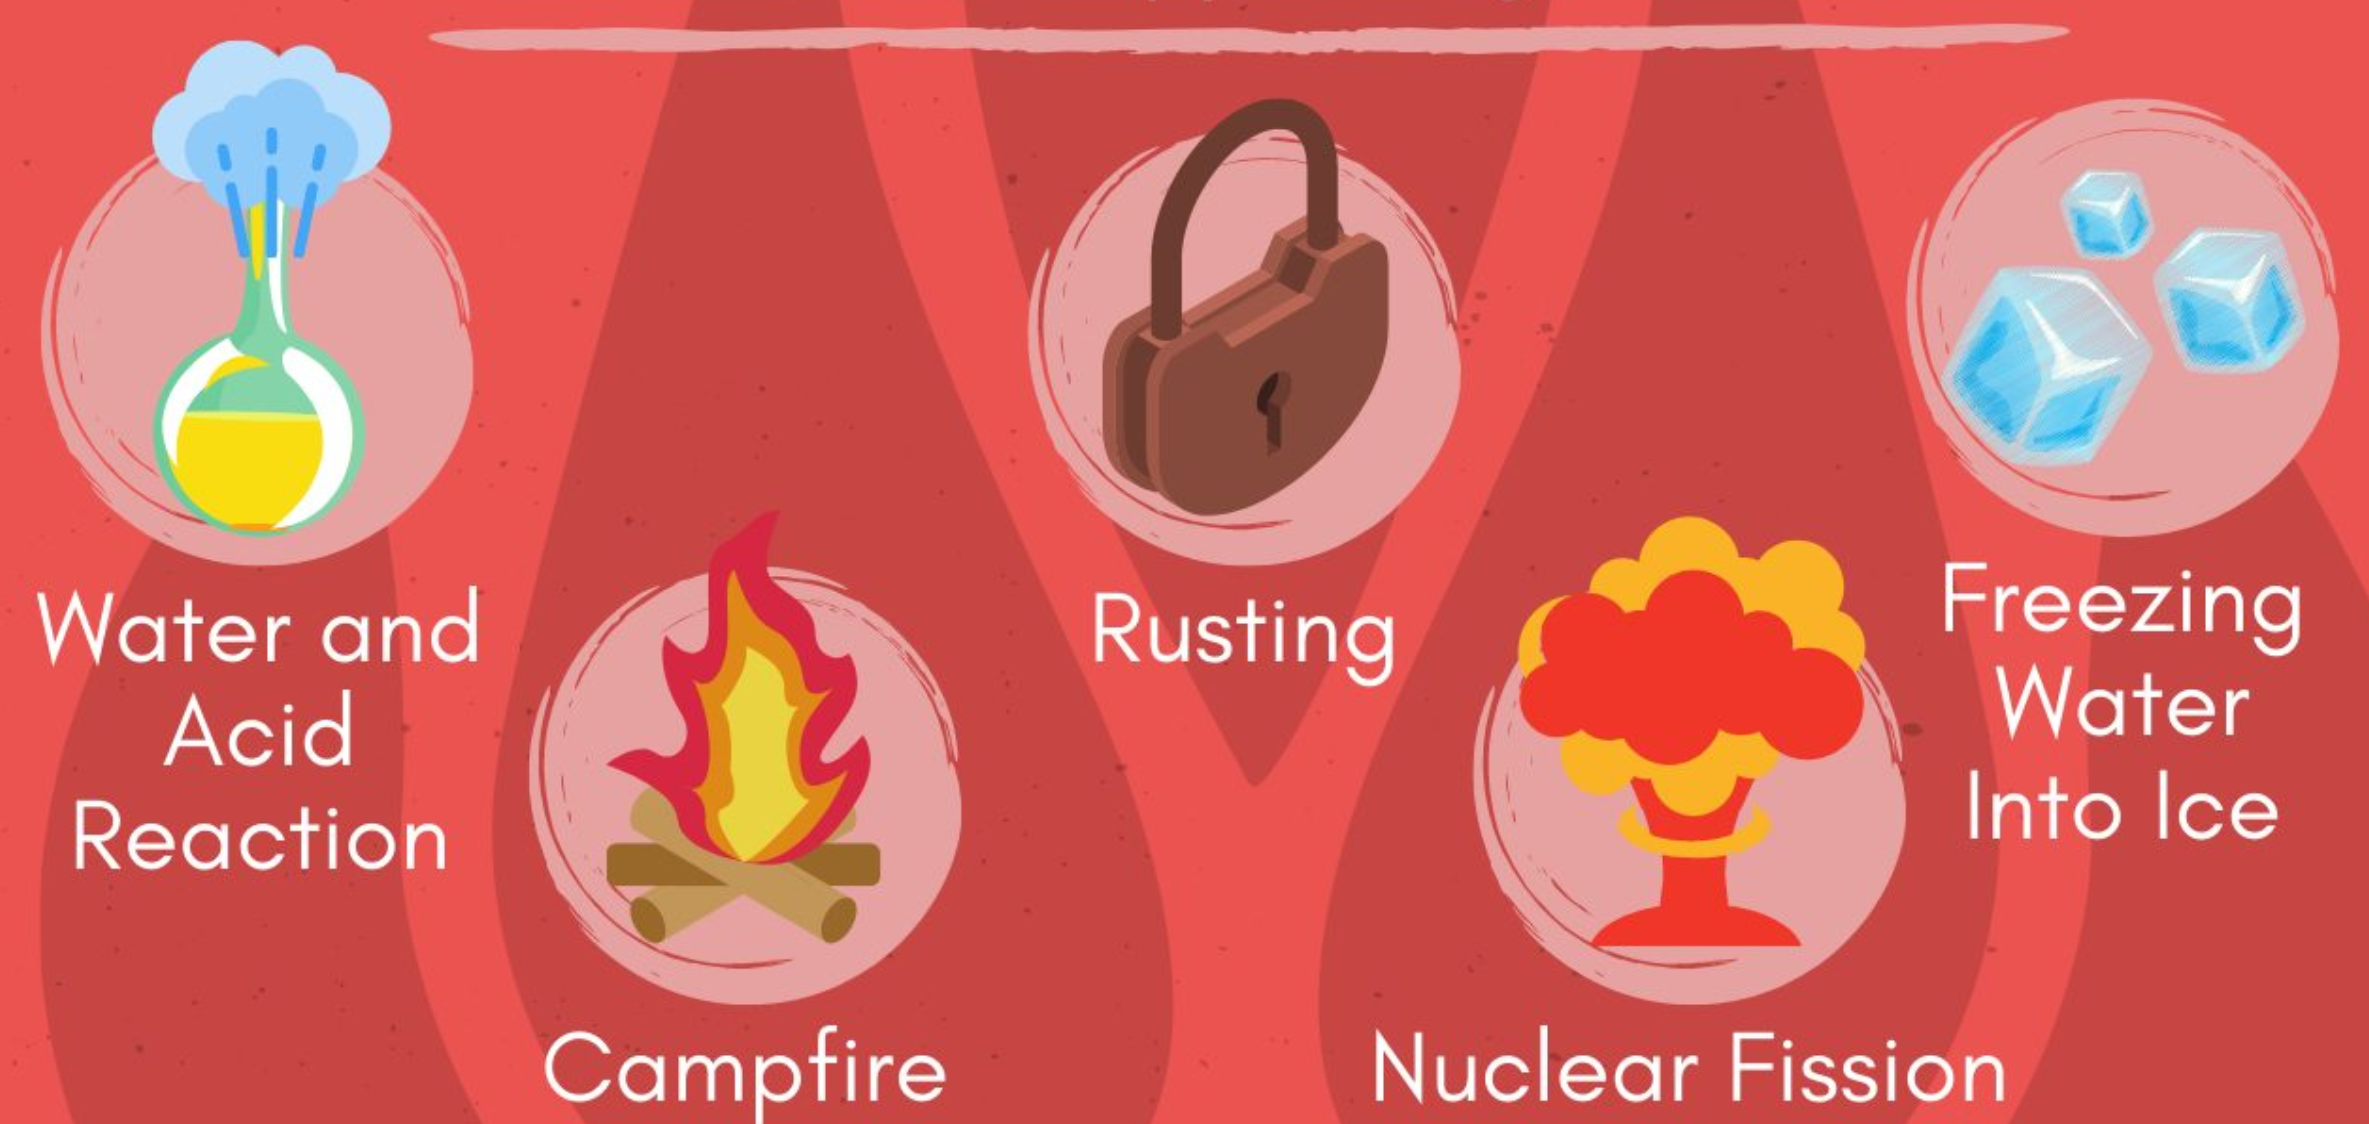
\includegraphics[width=\linewidth]{exo_everyday}
\end{frame}

\begin{frame}{Law of Conservation of Energy}
  \begin{center}
    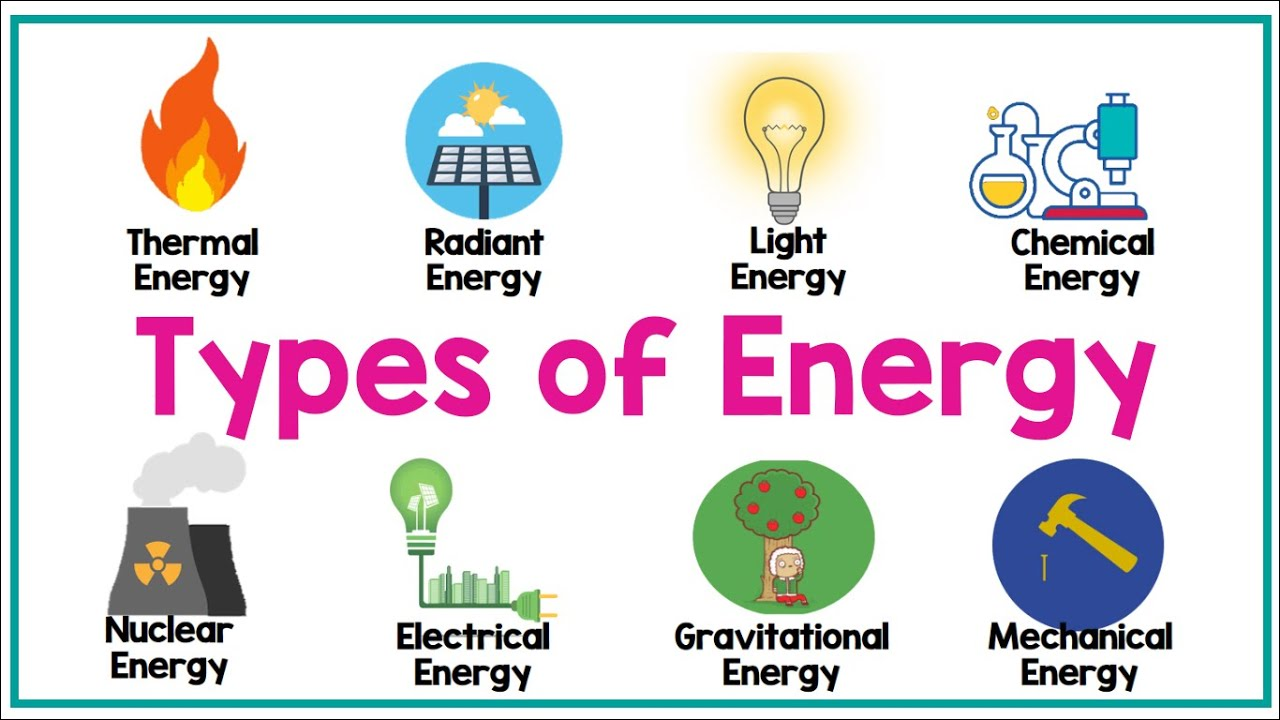
\includegraphics[scale=0.15]{energy_types}
    
    \textbf{Energy is neither created nor destroyed}
  \end{center}

  \begin{itemize}
  \item Energy can be converted from form to another
    e.g. mechanical, chemical, thermal, nuclear,
    electrical and vibrational energy
  \item Converting from one energy form to another is
    never $100\%$ efficient; there is always a loss of
    energy
  \end{itemize}
\end{frame}

\begin{frame}{Thermal Energy}
  \onslide<2->{\textbf{Thermal Equilibrium} - there is no ``net'' heat transfer}
  \centering
  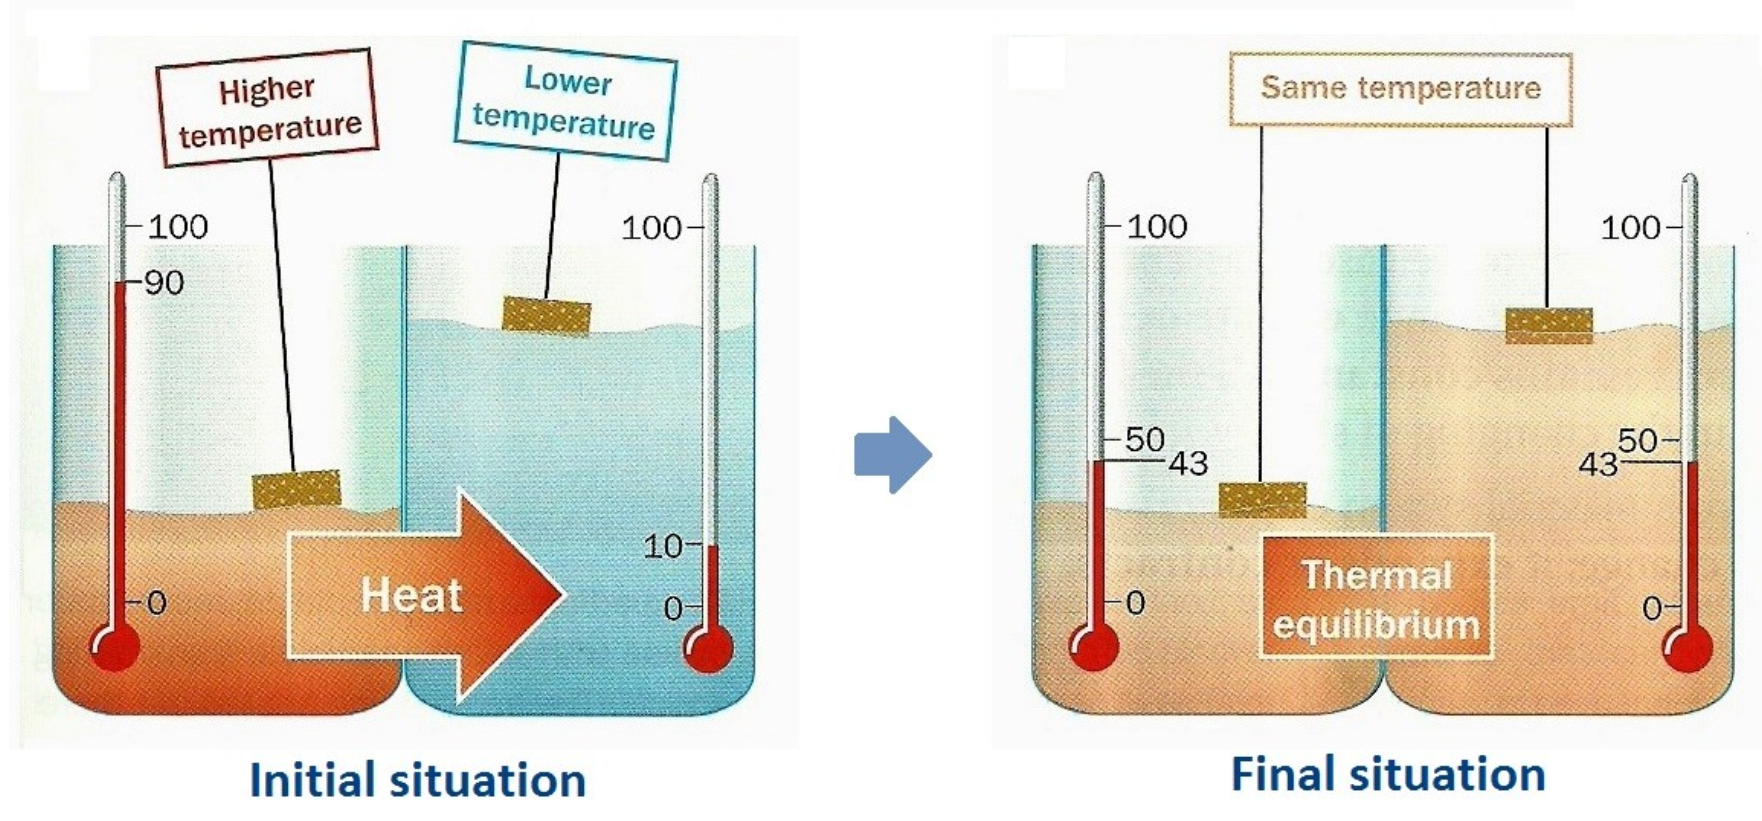
\includegraphics[width=\linewidth]{thermal_equil}

  Heat flows from ``hot'' to ``cold''
\end{frame}

\begin{frame}{Practice: Zeroth Law of Thermodynamics}
  \textbf{Q:} Suppose blocks A and C are in thermal equilibrium.
  In addition, blocks C and B are in thermal equilibrium as well.
  What conclusion can be drawn about the temperature of blocks A ($T_A$)
  and B ($T_B$)?
  
  \centering
  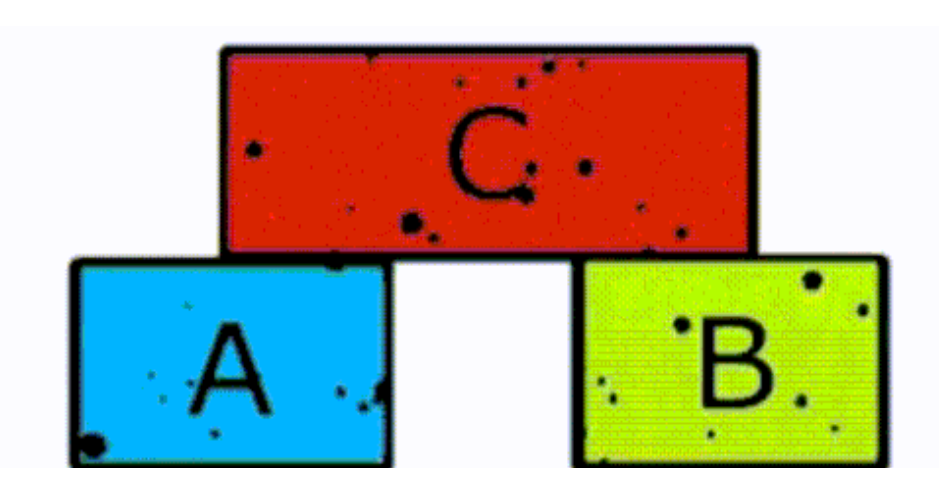
\includegraphics[width=0.7\linewidth]{zeroth_law}
\end{frame}

\begin{frame}{Zeroth Law of Thermodynamics}
  \begin{center}
    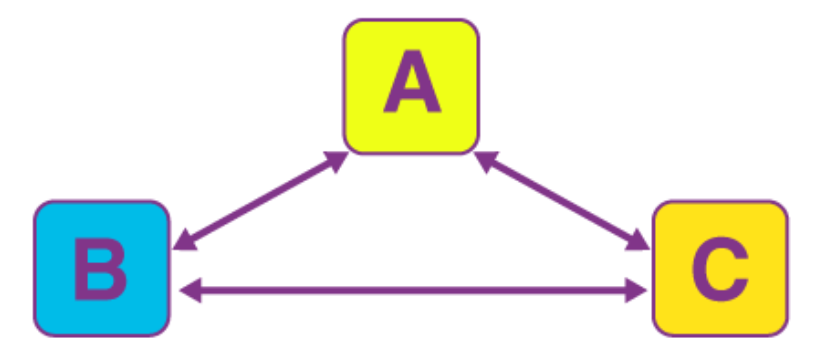
\includegraphics[width=0.7\linewidth]{trans_thermal}
  \end{center}

  ``If two thermodynamic systems are each in thermal equilirbium with a third one,
  then they are in thermal equilibrium with each other.''
\end{frame}

\begin{frame}{Quantifying Heat}
  \begin{equation}
    q = mC\Delta T
  \end{equation}
  where $q$ is heat, $m$ is the mass (g), $C$ is
  specific heat capacity (J/($^\circ$C g)) and $T$ is
  temperature ($^\circ$C)
\end{frame}

\begin{frame}{Practice: Thermal Equilibrium}
  Suppose there are two objects of the same material and mass.
  One is at a hot temperature $T_H$ and the second object is at a cold temperature
  $T_C$. Both come into contact and reach thermal equilibrium isolated from the
  surrounding. Determine the final temperature $T_f$.
  \vspace{1.2in}
\end{frame}

\begin{frame}{Practice: Thermal Equilibrium}
  Suppose there are two objects of the same material but one object is 2 times the
  mass of the other. One is at a hot temperature $T_H$ and the second object is at
  a cold temperature $T_C$. Both come into contact and reach thermal equilibrium
  isolated from the surrounding. Determine the final temperature $T_f$.
  \vspace{1.2in}
\end{frame}

\section{Review: Chemical Equation}

\begin{frame}{Meaning of a Chemical Equation}
  \begin{equation}
    aA + bB \rightarrow cC + dD
  \end{equation}
  where $a$, $b$, $c$, and $d$ are coefficients for the reactants $A$/$B$
  and products $C$/$D$
  
  \begin{itemize}
  \item Provides the means to determine how much product is
    produced for a given amount of reactants
  \item Relate to molar masses, number of molecules, amount
    of moles and masses
  \end{itemize}    
\end{frame}

\begin{frame}{Analogy to Recipe Cookbook}
  \begin{center}
    
\includegraphics[scale=0.11]{josh_weiss}
  \end{center}

  Analogy: \href{https://www.youtube.com/watch?v=T5SYu8tyKjM}{Cookbook recipe-
    Popeyes Chicken but better}
\end{frame}

\begin{frame}{Photosynthesis}
  \begin{equation}
    6\text{CO$_2$(g)} + 6\text{H$_2$O(l)} \rightarrow \text{C$_6$H$_{12}$O$_6$(s)}
    + 6\text{O$_2$(g)}
  \end{equation}

  \textbf{Properties}
  \begin{itemize}
  \item Balanced chemical equation satisfies the conservation of mass
  \item Coefficients in front of the molecules represent the relative
    moles of reactants and products
  \item \textbf{Q:} How many moles of H$_2$O(l) are needed to react with 12
    moles of CO$_2$(g)?
  \end{itemize}
\end{frame}

\begin{frame}{Practice: Acid-Base Reaction}
  Suppose you have 50mL of 1.5M HCl(aq) and you attempt to neutralize the
  acid with 1M NaOH(aq). Write the balanced chemical reaction. Determine
  what volume of 1M NaOH(aq) is needed.
  \vspace{1.2in}
\end{frame}

\begin{frame}{Approaching Limiting Reactant Problems}
  \begin{equation}
    \text{R1} + \text{R2} \rightarrow \text{P1}
  \end{equation}
  \begin{itemize}
  \item Given a certain amount of each reagents (R1 and R2)
    to produce P1, determine
    how much the R2 is needed to completely react with R1
  \item Based on that calculated value, determine whether
    there is enough R2 to completely react with R1
  \item If the amount of R2 is less than what is needed,
    then R2 is the limiting
  \item If the amount of R2 is more than what is needed,
    then R2 is the excess
  \end{itemize}
\end{frame}

\end{document}
